% Customizable fields and text areas start with % >> below.
% Lines starting with the comment character (%) are normally removed before release outside the collaboration, but not those comments ending lines

% svn info. These are modified by svn at checkout time.
% The last version of these macros found before the maketitle will be the one on the front page,
% so only the main file is tracked.
% Do not edit by hand!
\RCS$Revision: 132088 $
\RCS$HeadURL: svn+ssh://svn.cern.ch/reps/tdr2/papers/SMP-12-015/tags/July122012/SMP-12-015.tex $
\RCS$Id: SMP-12-015.tex 132088 2012-06-22 23:53:01Z kalanand $
%%%%%%%%%%%%% local definitions %%%%%%%%%%%%%%%%%%%%%
% This allows for switching between one column and two column (cms@external) layouts
% The widths should  be modified for your particular figures. You'll need additional copies if you have more than one standard figure size.
\newlength\cmsFigWidth
\ifthenelse{\boolean{cms@external}}{\setlength\cmsFigWidth{0.85\columnwidth}}{\setlength\cmsFigWidth{0.4\textwidth}}
\ifthenelse{\boolean{cms@external}}{\providecommand{\cmsLeft}{top}}{\providecommand{\cmsLeft}{left}}
\ifthenelse{\boolean{cms@external}}{\providecommand{\cmsRight}{bottom}}{\providecommand{\cmsRight}{right}}
\newcommand{\mjj}{\ensuremath{m_{jj}}\xspace}
\newcommand{\GeVnn}{\ensuremath{{\,\text{Ge\hspace{-.08em}V\hspace{-0.16em}}}}\xspace}
\newcommand{\GeVcnn}{\ensuremath{{\,\text{Ge\hspace{-.08em}V\hspace{-0.16em}}}}\xspace}
\newcommand{\GeVsnn}{\ensuremath{{\text{Ge\hspace{-.08em}V\hspace{-0.16em}}}}\xspace}
\newcommand{\mt}{\ensuremath{m_{\mathrm{T}}}\xspace}
\newcommand{\pb}{\ensuremath{\,\text{pb}}\xspace}
%%%%%%%%%%%%%%%  Title page %%%%%%%%%%%%%%%%%%%%%%%%
\cmsNoteHeader{SMP-12-015} % This is over-written in the CMS environment: useful as preprint no. for export versions
% >> Title: please make sure that the non-TeX equivalent is in PDFTitle below
\title{Measurement of WW and WZ production in W+dijet events in pp collisions}

% >> Authors
%Author is always "The CMS Collaboration" for PAS and papers, so author, etc, below will be ignored in those cases
%For multiple affiliations, create an address entry for the combination
%To mark authors as primary, use the \author* form
\address[cern]{CERN}
\author[cern]{The CMS Collaboration}

% >> Date
% The date is in yyyy/mm/dd format. Today has been
% redefined to match, but if the date needs to be fixed, please write it in this fashion.
% For papers and PAS, \today is taken as the date the head file (this one) was last modified according to svn: see the RCS Id string above.
% For the final version it is best to "touch" the head file to make sure it has the latest date.
\date{\today}

% >> Abstract
% Abstract processing:
% 1. **DO NOT use \include or \input** to include the abstract: our abstract extractor will not search through other files than this one.
% 2. **DO NOT use %**                  to comment out sections of the abstract: the extractor will still grab those lines (and they won't be comments any longer!).
% 3. **DO NOT use tex macros**         in the abstract: External TeX parsers used on the abstract don't understand them.
\abstract{
%% We report cross section measurement of 
%% simultaneous production of two gauge bosons  
%% diboson production 
%% in events 
%% containing a leptonically decaying W boson and exactly two jets.
%% The analyzed dataset 
%% corresponds to an integrated luminosity of 5.0~fb${}^{-1}$ at 
%% $\sqrt{s} = 7$~TeV collected by the CMS detector at the LHC.

We report a measurement of the diboson production 
cross section in events ontaining a leptonically decaying 
W boson and exactly two jets using 5.0~fb${}^{-1}$ data at 
$\sqrt{s} = 7$~TeV collected by the CMS detector at the LHC.
The measured value of the sum of WW and WZ cross sections is 
$66.70 \pm 8.08 \text{(stat)} \pm 8.52 \text{(syst)}$~pb, 
consistent with the standard model  prediction of 65.6~pb. 
This is the first observation of WW+WZ production using 
this signature in pp collisions. 
We find no evidence for anomalous triple gauge couplings 
and set upper limits on their magnitude.
%%Limits on anomalous triple gauge couplings
%%, extracted using 
%%the transverse momentum of the dijet system, 
%%show no significant deviation with respect to the SM prediction.
}

% >> PDF Metadata
% Do not comment out the following hypersetup lines (metadata). They will disappear in NODRAFT mode and are needed by CDS.
% Also: make sure that the values of the metadata items are sensible and are in plain text (no TeX! -- for \sqrt{s} use sqrt(s) -- this will show with extra quote marks in the draft version but is okay).

\hypersetup{%
pdfauthor={Kalanand Mishra},%
pdftitle={WW+WZ cross section in the W+dijet channel},%
pdfsubject={CMS},%
pdfkeywords={CMS, physics, software, computing}}

\maketitle %maketitle comes after all the front information has been supplied
% >> Text
%%%%%%%%%%%%%%%%%%%%%%%%%%%%%%%%  Begin text %%%%%%%%%%%%%%%%%%%%%%%%%%%%%
%% **DO NOT REMOVE THE BIBLIOGRAPHY** which is located before the appendix.
%% You can take the text between here and the bibiliography as an example which you should replace with the actual text of your document.
%% If you include other TeX files, be sure to use "\input{filename}" rather than "\input filename".
%% The latter works for you, but our parser looks for the braces and will break when uploading the document.
%%%%%%%%%%%%%%%
%%\section{Introduction}
The pair production of vector bosons allows to directly 
test their self-interactions predicted by the 
gauge symmetry of the standard model (SM)~\cite{PhysRevD.48.2182}. 
Observations of anomalous couplings would be an indication of new physics.
Also, Higgs boson may decay to WW, giving rise to the same 
final state as in diboson production. 


In this Letter we report the first observation of diboson 
production in the semi-leptonic final state at a pp collider.
One W boson decays leptonically while the other boson 
(W or Z) decays hadronically giving rise to two energetic jets in 
the final state.
Previous measurements in this channel at the Tevatron p$\overline{\rm p}$ 
collider include the recent CDF~\cite{CDF-diboson-lvjj-2010} and 
D\O~\cite{Abazov:2011cb} results. 
The advantage of reconstructing WW+WZ in $\ell\nu jj$ decay mode over 
the purely leptonic final states is the larger branching fraction to jets, 
at the expense of larger backgrounds, mainly from W+jets.
Compared to the pure WW leptonic diboson decay the semi-leptonic 
process has the ability to  provide a direct handle on the boson transverse 
momentum. 
The sensitivity to very high boson $p_T$ makes this process particularly 
useful as a probe of the gauge symmetries at high energies 
where we anticipate new physics.




Our data correspond to an integrated luminosity of $5.02 \pm 0.11\fbinv$ 
collected with the CMS detector in pp collisions at $\sqrt{s} = 7\TeV$ at
the CERN LHC in 2010 and 2011.
CMS~\cite{CMS:2010} uses a right-handed coordinate system, with the origin at the nominal
interaction point, the x-axis pointing to the center of the LHC, the y-axis pointing up
perpendicular to the LHC plane, and the z-axis along the counterclockwise-beam direction. The polar
angle $\theta$ is measured from the positive z-axis and the azimuthal angle $\phi$ is measured in
the x-y plane. The pseudorapidity is defined as $\eta = -\ln(\tan\frac{\theta}{2})$.
The CMS detector~\cite{CMS:2010} consists of pixel and silicon-strip trackers up to $|\eta| < 2.5$
which, together with a 3.8 Tesla solenoid, provide
a track momentum resolution of 1\% at 100\GeVnn; a granular electromagnetic crystal-calorimeter  
extending up to $|\eta| < 3$ with an energy resolution of about $3\%/\sqrt{E}$ 
\cite{CMS-PAS-EGM-10-003}; a hadronic
calorimeter extending up to $|\eta| < 5$ with
an energy resolution of $100\%/\sqrt{E}$; and an efficient muon system capable of reconstructing and
identifying muons up to $|\eta| < 2.4$. The detector is nearly hermetic, allowing for measurements
of the missing transverse energy ($\MET$) in the event. 
A two-tier trigger system selects the events for use in
physics analysis.



We use data collected with a suite of single lepton triggers mostly 
using transverse momentum (\PT) thresholds of 24\GeVnn for muons 
and $25-32$\GeVnn for electrons. To preferentially keep only real W
events, the single electron triggers typically also require minimum 
thresholds on $\MET$ and the
transverse mass \mt of the electron plus $\MET$ system. 
The overall trigger efficiency is about 94\% (90\%) for muon (electron) data, 
with a small dependence (within a few percent) on \PT and $\eta$. 
Simulated Monte Carlo (MC) samples are corrected for the trigger efficiency.
Although the main sources of background are estimated from data, 
Monte Carlo simulations are used to
develop and validate the methods used in the analysis. 
We use the \MADGRAPH~\cite{MADGRAPH} event
generator and CTEQ6L1 parton distribution functions to simulate the 
W boson and Drell-Yan production
in association with up to four jets at the level of matrix element (ME) 
calculation and matched to
parton showers (PS) from \PYTHIA 6.422~\cite{PYTHIA} tune 
Z2~\cite{Collaboration:2012tb} with a matching
threshold of 20\GeVnn and a dynamic factorization/renormalization scale given by
{\small $\sqrt{m^{2}_{\textnormal{W/Z}} + p^{2}_{\textnormal{T, W/Z}}}$}.
Top-quark pair events are also simulated using \MADGRAPH. 
Single top production is modeled using
\POWHEG~\cite{Nason:2004rx,Frixione:2007vw,Alioli:2010xd,Nason:2009ai}. 
Multi-jet and electroweak diboson WW and WZ 
processes are simulated using \PYTHIA. 
All MC events are fully reconstructed using the standard CMS software.






Muons are measured with the all-silicon tracker and the muon system, 
within $|\eta|<2.1$. Electrons are detected as tracks in the tracker 
pointing to energy clusters in the ECAL, within $|\eta|<2.5$, 
excluding the transition region between the barrel and endcap, 
$1.44<|\eta|<1.57$. Muons (electrons) are required to have a momentum 
transverse to the beam direction, \PT, greater than 25\GeVnn
(35\GeVnn).
To reduce the background from processes that do not contain 
$\textnormal{W}\to\ell\nu$ decays, we require that the transverse 
mass~\cite{VBTF} of the W candidate be larger than 30\GeVnn (50\GeVnn) 
in muon (electron) data.
The lepton candidates are required to be compatible with the primary 
vertex of the event, which is chosen as the vertex with highest 
$\sum \PT^2$ of its associated tracks. According to the simulation,
this requirement provides the correct assignment for the primary 
vertex in more than 99\% of cases
in both signal and background simulated events. Charged leptons from 
W boson decays are expected to
be isolated from other activity in the event.
Leptons are therefore required to be isolated from hadronic activity 
in the detector by restricting
the sum of transverse momentum or energy in the tracker, ECAL, and HCAL, 
within a surrounding cone
of $\Delta R \equiv \sqrt{(\Delta\eta)^2+(\Delta\phi)^2} <0.3$, to be 
less than 10\% of the measured
$\PT$ of the muon, or less than 5\% of the measured $\PT$ of the electron, 
where $\Delta\eta$ and
$\Delta\phi$ are the differences in pseudorapidity and in azimuthal angle 
in radians.
To reduce the backgrounds from the Drell-Yan and electroweak diboson 
purely-leptonic decay processes, we veto the presence of any other 
loosely identified lepton (of $\PT > 20\GeVnn$ for electron,
10\GeVnn for muon) in the event.


Jets are reconstructed from calorimeter and tracker information 
using a particle flow technique~\cite{CMS-PAS-PFT-09-001}. 
The anti-\kt clustering algorithm~\cite{antikt,fastjetmanual} with 
distance parameter ${\rm R=0.5}$ is used. 
Jets that overlap with isolated leptons within $\Delta R=0.3$ are 
not considered.
Jet-energy corrections are applied to account for the non-linear 
response of the calorimeters to the particle energies and other 
instrumental effects~\cite{jetpas}. 
These corrections are based on in-situ measurements using di-jet, 
$\gamma+{\rm jet}$, and Z+jet data samples~\cite{Chatrchyan:2011ds}.
Overlapping minimum-bias events coming from different proton-proton 
collisions (pile-up) and the underlying event have an effect on jet 
reconstruction by contributing additional energy to the reconstructed jets. 
The median energy density due to pile-up is evaluated in each event and the
corresponding energy is subtracted from each jet~\cite{Cacciari:2008gn}.
A jet quality requirement, primarily based on the energy balance between 
charged and neutral hadrons in a jet, is applied to remove misidentified jets. 
A selection requirement $\PT>35\GeVnn$ is applied to all jets. 
Only events with two jets above this threshold within the tracker acceptance
($|\eta|<2.4$) are selected for the analysis.
An accurate $\MET$  measurement is essential for distinguishing the 
W signal from QCD backgrounds and to reconstruct the full event 
kinematics of the WW system. 
We use $\MET$ measured in the event using the full particle-flow 
reconstruction~\cite{Chatrchyan:2011tn}. 
%%The $\MET$ resolution, measured as a
%%function of the sum $\ET$ ($\sum\ET$) of the particle-flow objects in the
%%event, varies from 4\% at $\sum\ET=60\GeVnn$ to 10\% at 
%%$\sum\ET=350\GeVnn$~\cite{Chatrchyan:2011tn}.
We require $\MET>25$ (30)\GeVnn in the event in case of muon (electron) data.





We determine the relative contribution of the known SM processes to
the observed \mjj spectrum using an unbinned maximum likelihood fit in
the range between 40~GeV and 200~GeV.  The fit is performed separately
for the electron and muon channels and for the 2-jet and 3-jet
samples since relative background compositions differ.
%%%%%%%%%%%%%%%%%%%%%%%%%%%%%%
\begin{table}[bt]
 \caption{Determination of the \mjj shape and normalization. External constraints are assumed Gaussian.}  
 \label{tab:Table0} 
\begin{ruledtabular}
\begin{tabular} {lcl}
   Process             &    Shape     & Constraint on normalization \\ 
   \hline
   Diboson             &    MC        & Unconstrained \\ 
   W plus jets         &    MC        & (approx NLO) 31314 pb $\pm$ 5\%~\cite{MCFM} \\
   \ttbar\             &    MC        & (approx NLO) 163 pb $\pm 7\%$~\cite{Kidonakis:2010dk}\\ 
   Single top          &    MC        & (approx NNLO) $\pm 5\%$~\cite{Kidonakis:2010tc,Kidonakis:2011wy,Kidonakis:2010ux}\\
   Multijet            &    data      & \met fit in data (see text) \\
   Drell-Yan + jets    &    MC        & (NNLO) 3.05 nb $\pm 4.3\%$~\cite{FEWZ} \\  
 \end{tabular}
\end{ruledtabular}
\end{table}
%%%%%%%%%%%%%%%%%%%%%%%%%%%%%%
Table~\ref{tab:Table0} lists the SM processes included in the fit.
The normalization of the diboson WW+WZ contribution is a free
fit parameter. The normalizations of the background components
are allowed to vary within a Gaussian constraint around their central
values. For multijet events, this central value is obtained from a
separate fit to the $\met$ distribution~\cite{VBTF}, and the
constraint is driven by the corresponding fit error estimate. The
central values for all other processes are obtained from
next-to-leading order (NLO) or next-to-NLO (NNLO) calculations, and
the constraints reflects the theoretical uncertainties.  With the
exception of multijet production, the \mjj template distribution
shapes for all processes are obtained from simulation.  Multijet
events contribute when jets are misidentified as isolated
leptons. Hence their \mjj shape can be derived from data events with
lepton candidates that fail the isolation requirements.


The \mjj spectrum of the dominant W plus jets component is 
described using \MADGRAPH shape after taking into account 
the uncertainties due to the factorization/ renormalization scale 
($q$) and ME--PS matching scale $\mu$:
\begin{linenomath}
\begin{align}
\mathcal{F}_{\text{W+jets}} = \alpha &\cdot \mathcal{F}_{\text{W+jets}} (\mu_{0}^2, q'^2) + 
\beta \cdot \mathcal{F}_{\text{W+jets}} (\mu'^2, q_{0}^2) \nonumber \\ 
&+ (1-\alpha-\beta) \cdot \mathcal{F}_{\text{W+jets}} (\mu_{0}^2, q_{0}^2)\,,
\label{eqWpjetsShape}
\end{align}
\end{linenomath}
where $\mathcal{F}_{\text{W+jets}}$ denotes the \mjj shape from
simulation.  The parameters $\mu_0$ ($\mu'$) and $q_0$ ($q'$)
correspond to the default (alternative) values of $\mu$ and $q$
respectively, and fractional contributions $\alpha$ and $\beta$ are
free to vary in the fit.  We take $\mu' = 2 \mu_0$, if $\beta>0$ and
$\mu' = 0.5 \mu_0$, if $\beta<0$; similarly, $q' = 2 q_0$, if
$\alpha>0$ and $q' = 0.5 q_0$, if $\alpha<0$.
%%%%%%%%%%%%%%
\begin{figure*}[tbh]
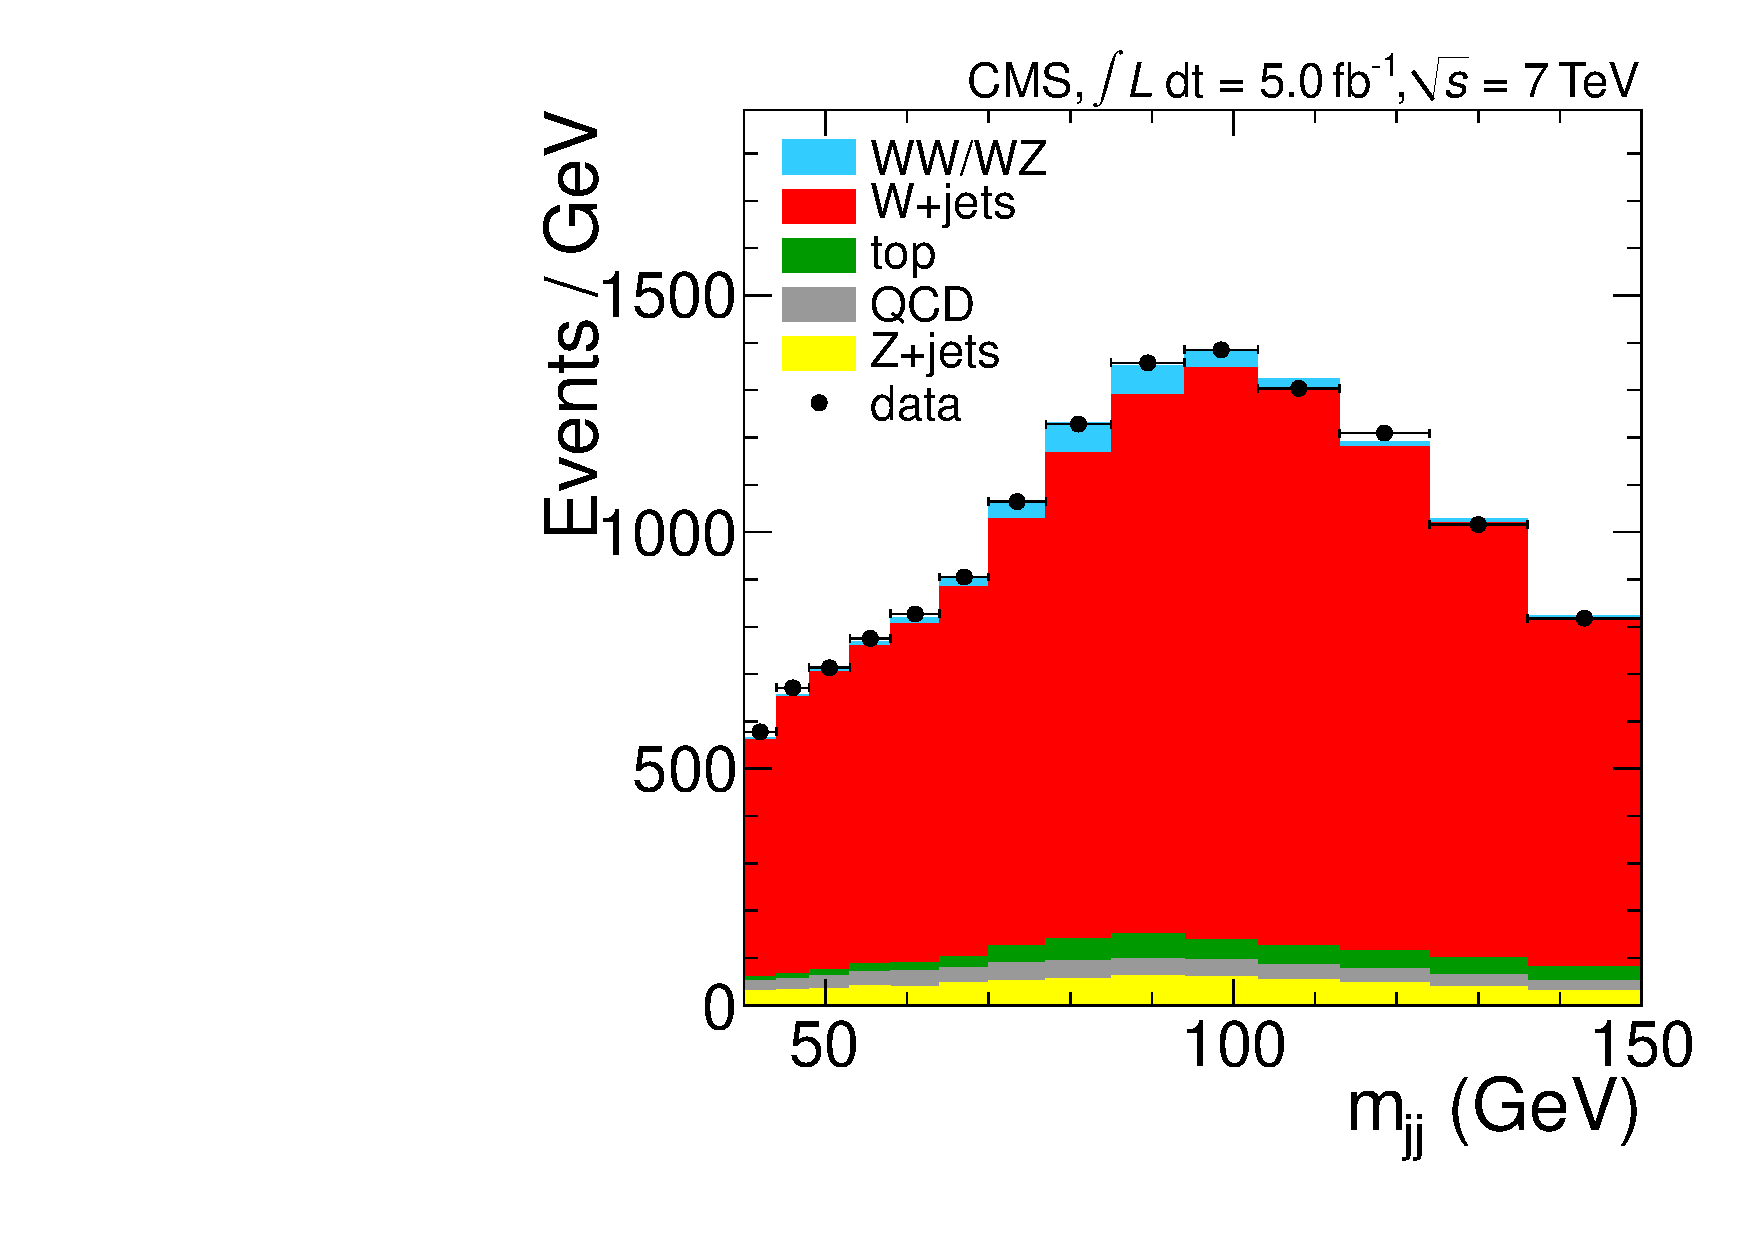
\includegraphics[width=0.3\textwidth]{figs/Diboson_Stacked_combined}
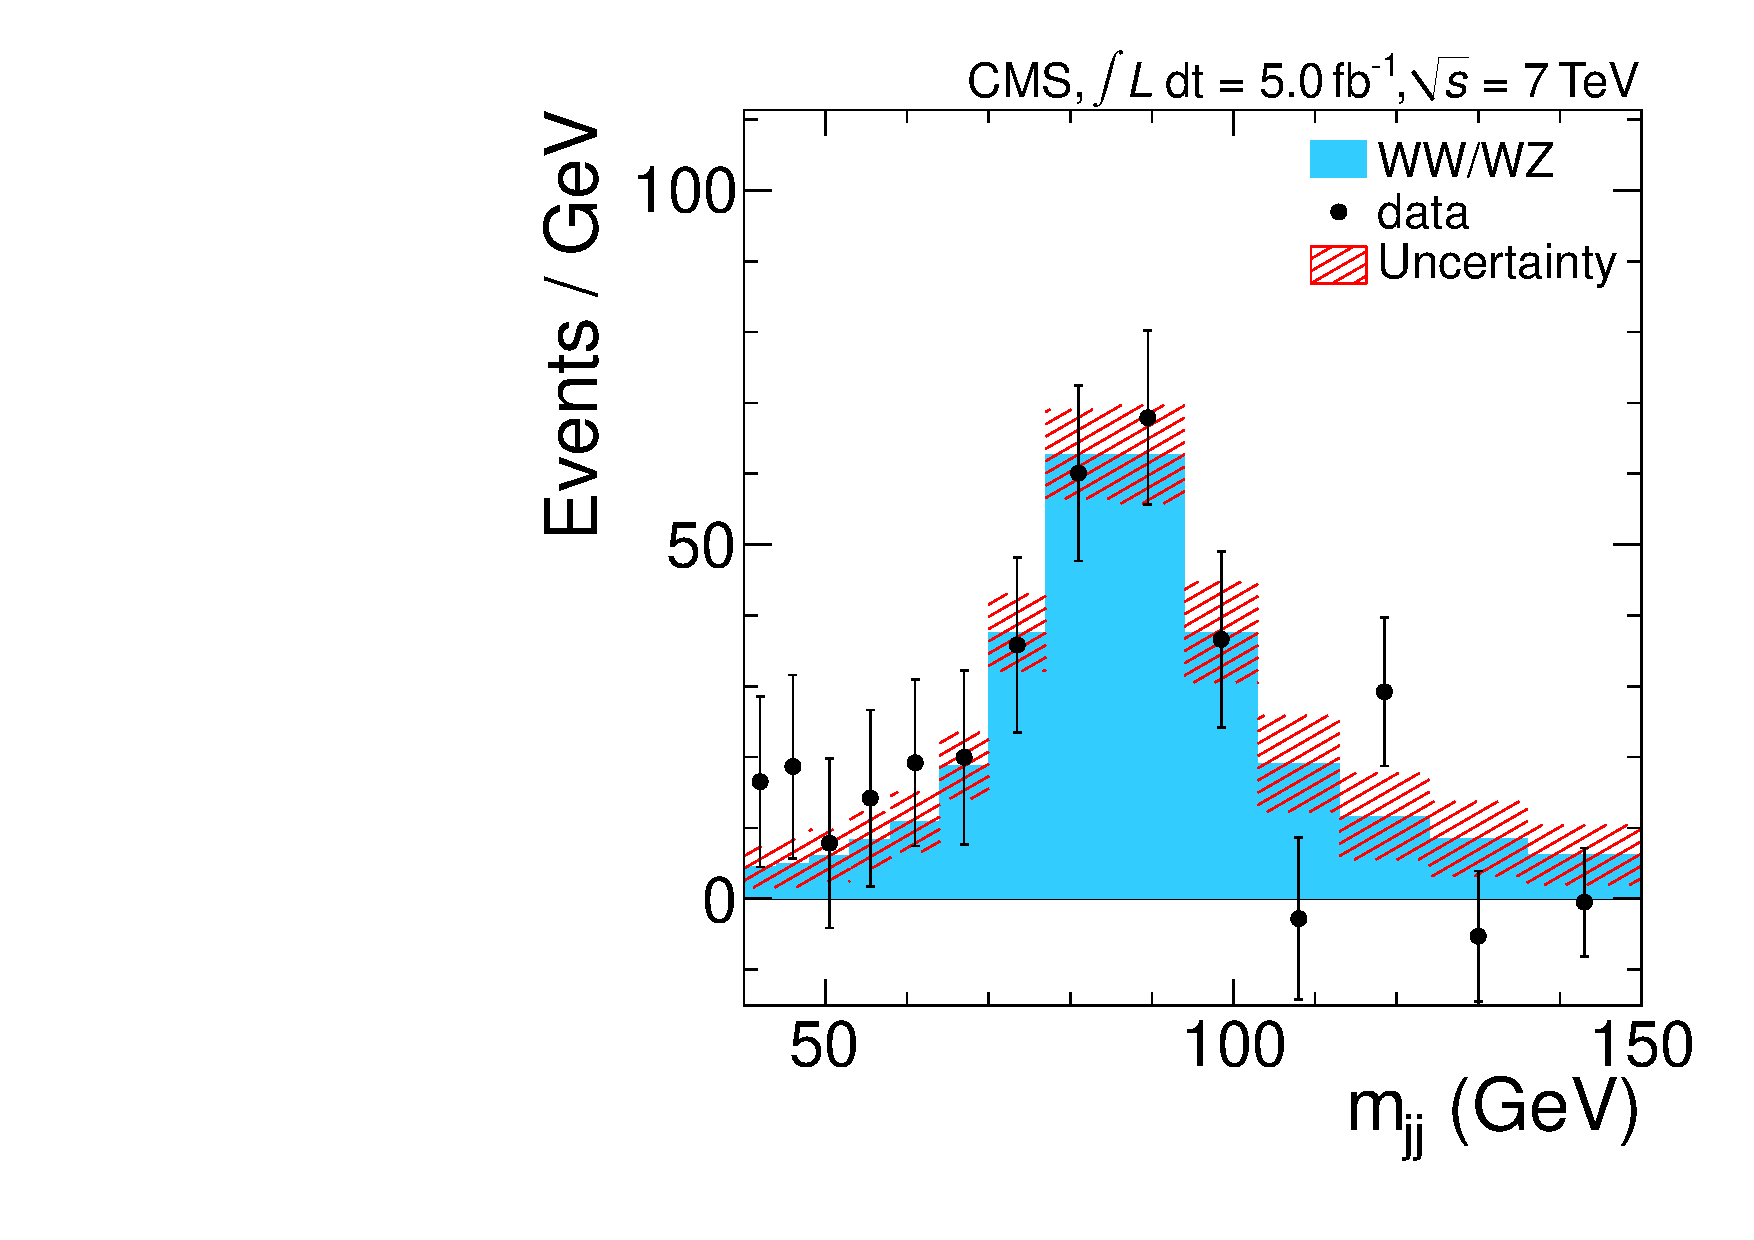
\includegraphics[width=0.3\textwidth]{figs/Diboson_Subtracted_combined}
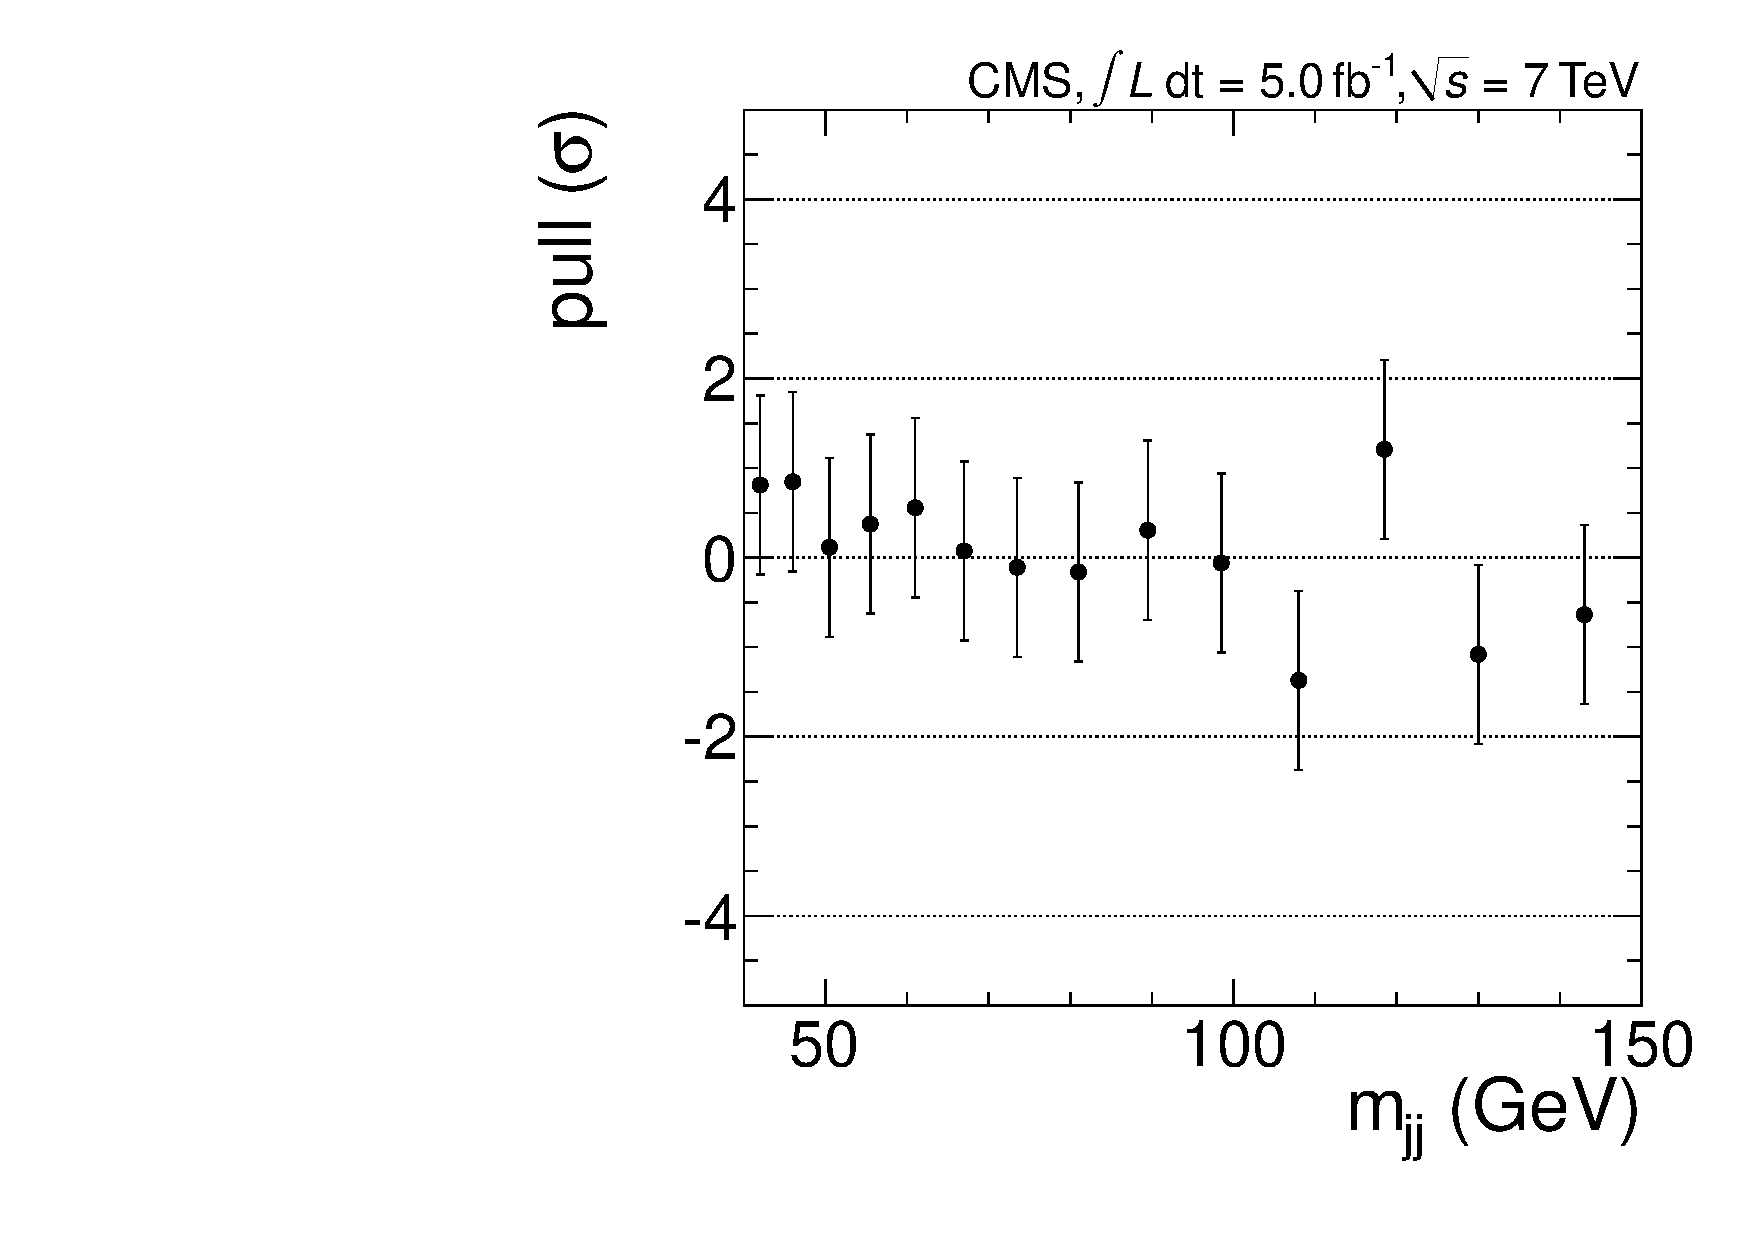
\includegraphics[width=0.3\textwidth]{figs/Diboson_Pull_combined}
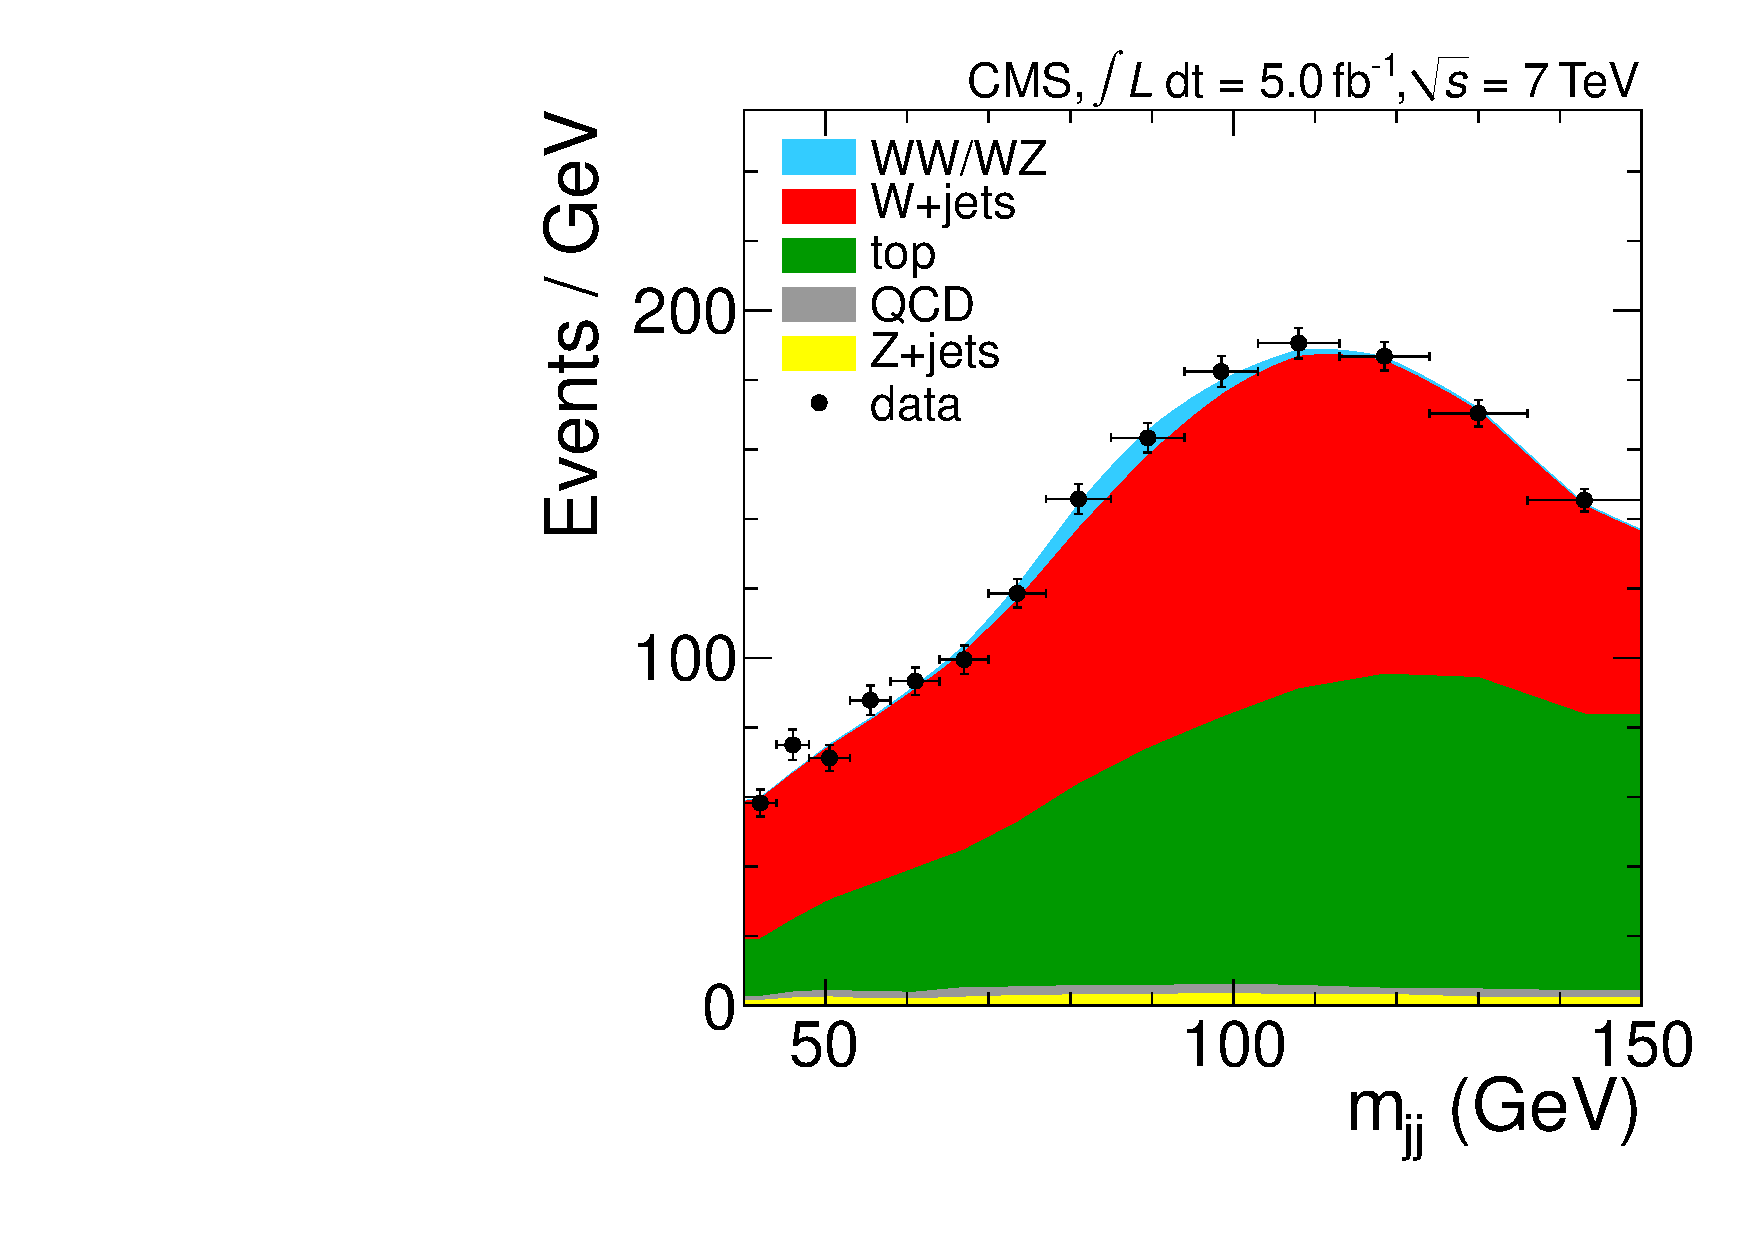
\includegraphics[width=0.3\textwidth]{figs/Diboson_btag_Stacked_combined}
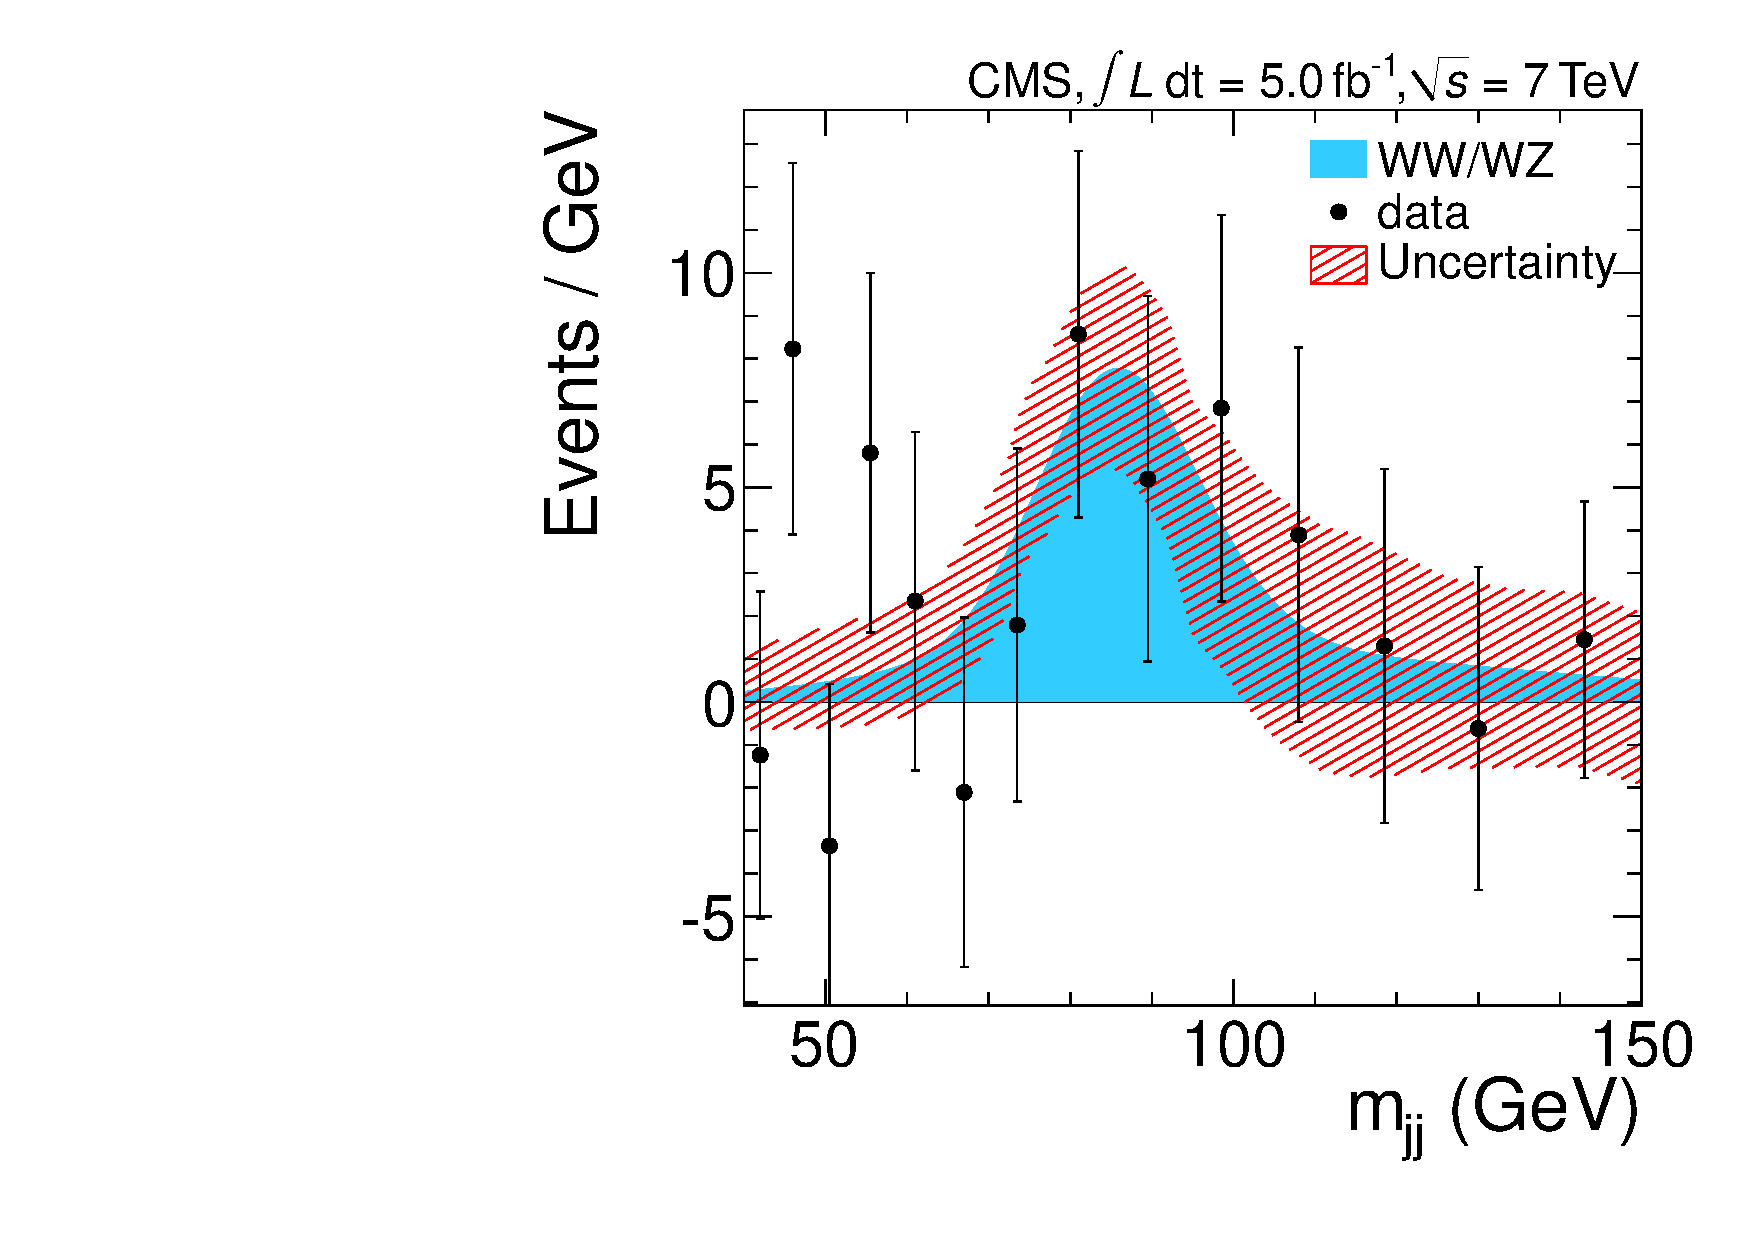
\includegraphics[width=0.3\textwidth]{figs/Diboson_btag_Subtracted_combined}
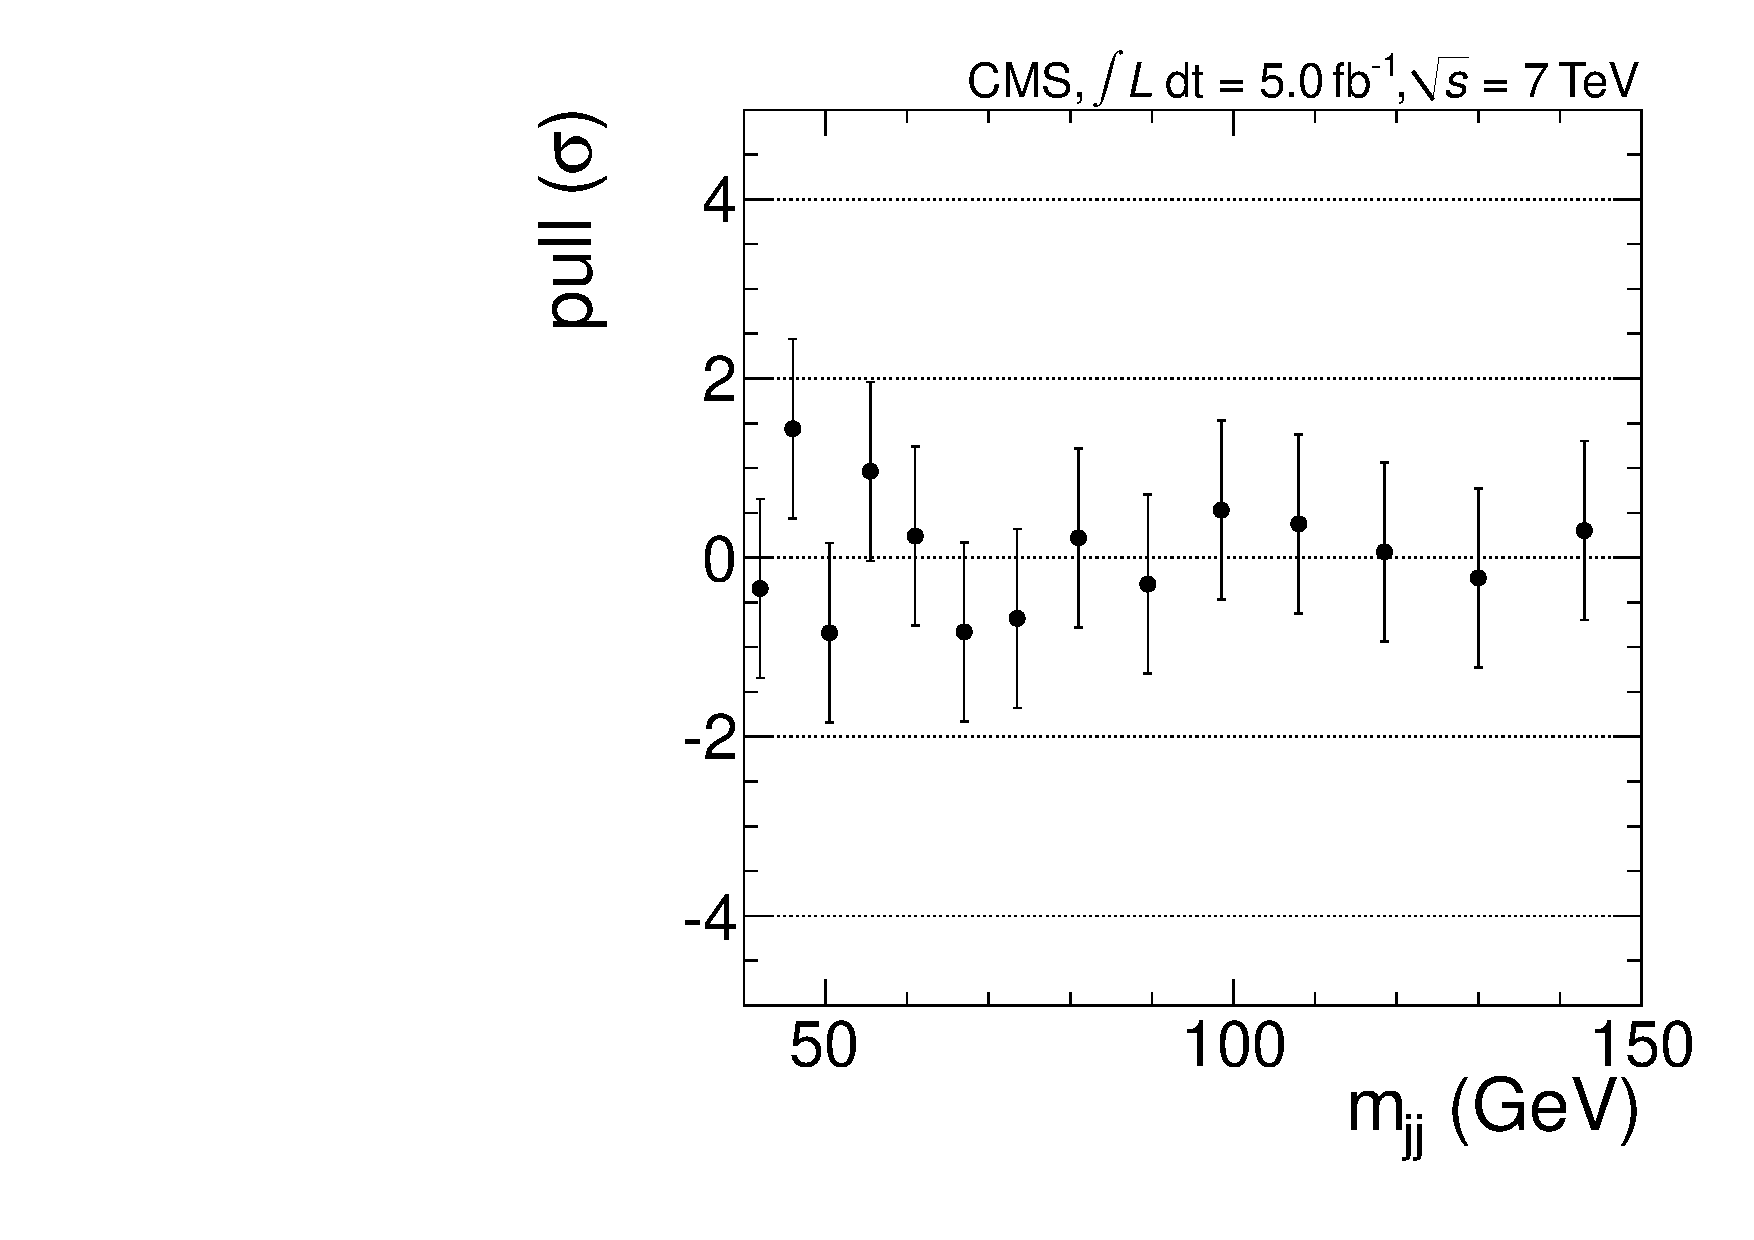
\includegraphics[width=0.3\textwidth]{figs/Diboson_btag_Pull_combined}
\caption{(a, d) Distribution of the dijet invariant mass in data. 
Overlaid are the fit projections of various components. Depicted is the
number of events per GeV, \textit{i.e.}, the event count divided by bin width.  
(b, e) The same
distribution after subtraction of all components except the
diboson.  Error bars correspond to the
statistical uncertainty and the band represents the systematic
uncertainty .  (c, f) Normalized
residual: $(\text{data} - \text{fit})/\text{uncertainty}$. 
The plots in the upper (lower) row are for muon (electron) data 
after combining the ``no b-tag'' and ``b-tag'' categories.
}
\label{fig:Fig1}
\end{figure*}
%%%%%%%%%%%%%%
%%%%%%%%%%%%%%%%%%%%%%%
\begin{table*}[htbp]
  \caption{Event yields determined from a likelihood fit to the data. 
  The total uncertainty includes the effect of correlation among the 
  individual contributions using the full covariance matrix.}
  \label{tab:yields}
\begin{ruledtabular}
  \begin{tabular} {lllll}
                       &    \multicolumn{2}{c}{Muon channel} & \multicolumn{2}{c}{Electron channel} \\
    Process            &    no b-tag         &  b-tag         &  no b-tag          &  b-tag\\
\hline
        Diboson (WW+WZ) &   1736 $\pm$ 389       &  226 $\pm$ 203   &  727 $\pm$ 302   &   35 $\pm$ 86 \\
        W plus jets     &   67674 $\pm$ 586      &  5082 $\pm$ 206  & 32706 $\pm$ 850  & 2693 $\pm$ 107 \\
        Single top      &   652 $\pm$ 33         &  1219 $\pm$ 60   &  332 $\pm$  17   &  626 $\pm$ 31 \\
        $\ttbar$        &   1666 $\pm$ 117       &  3192 $\pm$ 191  &  953 $\pm$  67   & 1976 $\pm$ 104 \\
        Multijet  (QCD) &   119 $\pm$ 317        &  16 $\pm$ 42     & 3204 $\pm$ 867   &  231 $\pm$ 78 \\
        Drell-Yan plus jets (Z+jets) &   3613 $\pm$ 155   &  206 $\pm$ 9     &  1485 $\pm$ 64   &  858 $\pm$ 37 \\
\hline
%   Fit $\chi^2$ probability&   0.454        & 0.729           &  0.969           & 0.991    \\
    Total from fit      &    75460           &  9941               &  39407           & 5648  \\
    Data                &    75419           &  9940               &  39365           & 5695 \\
\hline
    Acceptance $\times$ efficiency & $5.153 \times 10^{-3}$ & $6.402 \times 10^{-4}$ & $2.633 \times 10^{-3}$ & $3.332 \times 10^{-4}$\\
  \end{tabular}
\end{ruledtabular}
\end{table*}
%%%%%%%%%%%%%%
Figure~\ref{fig:Fig1}(a) shows the observed \mjj distribution for all
four channels combined, together with the fitted projections of the
contribution of various SM processes.  Figure~\ref{fig:Fig1}(b)
shows the same distribution after subtracting all SM contributions
from data except for electroweak diboson WW+WZ events.  
Figure~\ref{fig:Fig1}(c) shows the normalized
residual, \textit{i.e.}, pull distribution defined as $(\text{data} -
\text{fit})/\text{uncertainty}$.  Table~\ref{tab:yields} presents the
yields of various SM components obtained from the fit. 


We validate the fit procedure by performing pseudo-experiments.  In
each experiment, we generate the \mjj pseudo-data of the SM processes,
taking into account the correlation among the yields, and then fit
each pseudo-data sample.  The results indicate that the bias on the
diboson yield is below 0.4 standard deviations and that the 
fit overerstimates the yield
uncertainty slightly. These effects are corrected for in the final
result.  Uncertainties in the jet energy are estimated in a sample of
W bosons decaying hadronically in a highly pure sample of semileptonic
\ttbar\ events.  The mean and resolution of the reconstructed dijet
(\textit{i.e.,} W) mass distribution in data agree within 0.6\% with
the expectation from simulation.  A small difference in \met
resolution~\cite{Chatrchyan:2011tn} between data and simulation
affects the signal acceptance at the 0.5\% level.  
Further systematic uncertainties
are due to the uncertainty of the trigger efficiency estimates in
data, which is 1\%, and the estimate of lepton reconstruction and
selection efficiency, which is 2\%~\cite{VBTF}.  The uncertainty
in the luminosity determination is 2.2\%~\cite{lumiPAS}.
Theoretical uncertainty in acceptance computation is 4\%. 


With the kinematic requirements imposed in the analysis, we 
observe 2979 $\pm$ 361 (stat) $\pm$ 402 (syst) WW+WZ events, 
in agreement with the Standard Model expectation. 
We compute the WW+WZ cross section as 
$\sigma = N^{\text{Sig}}/ (\cal{A} \, \varepsilon \, {\cal{L}})$, 
 where $N^{\text{Sig}}$ is the number of extracted signal events,
$\cal{A}$ is the signal acceptance corrected for the branching fractions,
$\varepsilon$ is the efficiency for all requirements on 
the event selection, and ${\cal{L}}$ is the integrated luminosity.
The values of $N^{\text{Sig}}$ and $\cal{A} \times \varepsilon$ 
are given in Table~\ref{tab:yields} for each data category. 
Combining all four categories, we obtain: 
$\sigma = 66.70 \pm 8.08 \text{(stat)} \pm 8.52 \text{(syst)}$~pb, 
which is in agreement with the NLO prediction~\cite{Campbell:2011bn} 
$65.6 \pm 2.2$~pb.


The $s$-channel production of WW events occurs via triple-gauge couplings 
WW$\gamma$ and WWZ, while the corresponding WZ production occurs via  
WWZ couplings. 
%%In the SM, these couplings are defined  up to an overall constant. 
Contributions to these couplings from new physics processes would 
affect the measured WW+WZ cross section and the kinematic 
distributions~\cite{PhysRevD.48.2182}. 
We search for anomalous gauge couplings using an effective 
Lagrangian described by the HISZ parametrization~\cite{PhysRevD.48.2182} 
without form factors.
We find no evidence for anomalous couplings 
and set upper limits on their magnitude.
Given the tight bound on parameter $\Delta{g_1^Z}$~\cite{pdg} 
we assume the SM value, \ie 0, for it and set limits on 
the other two parameters $\Lambda_\gamma$ and $\Delta{\kappa_Z}$.  
We use dijet $p_T$ distribution, shown in Fig.~\ref{fig:Fig2}a, 
as the observable after requiring  $75~\GeVnn < \mjj < 95~\GeVnn$. 
The dependence of the distribution on specific anomalous couplings 
is modeled by re-weighting the Pythia simulation of WW+WZ to 
the MCFM~\cite{MCFM} predictions. 
We account for systematic uncertainties due to the 
normalization and shape of the SM processes, 
quoted luminosity, signal selection efficiency, and signal shape. 
Upper limits in 2-dimensional $\Lambda_Z:\Delta{\kappa_\gamma}$ plane
computed using CL${}_{S}$~\cite{CLS} with LHC test statistic are shown in 
Fig.~\ref{fig:Fig2}b. At the 95\% confidence level  
we obtain the following observed upper limits: 
$ -0.038 < \Lambda_Z < 0.030$, $ -0.11 < \Delta{\kappa_\gamma} < 0.14$.
These limits are the most stringent at a hadron collider to-date. 
%%The corresponding expected exclusion limits are
%%$ -0.041 < \Lambda_Z  < 0.035$, $ -0.12 < \Delta{\kappa_\gamma} < 0.16$.
%%These limits are consistent with the SM prediction. 
%%%%%%%%%%%%%%%%%%%%%%%%%%%%
\begin{figure}[tbh]
  {\centering
    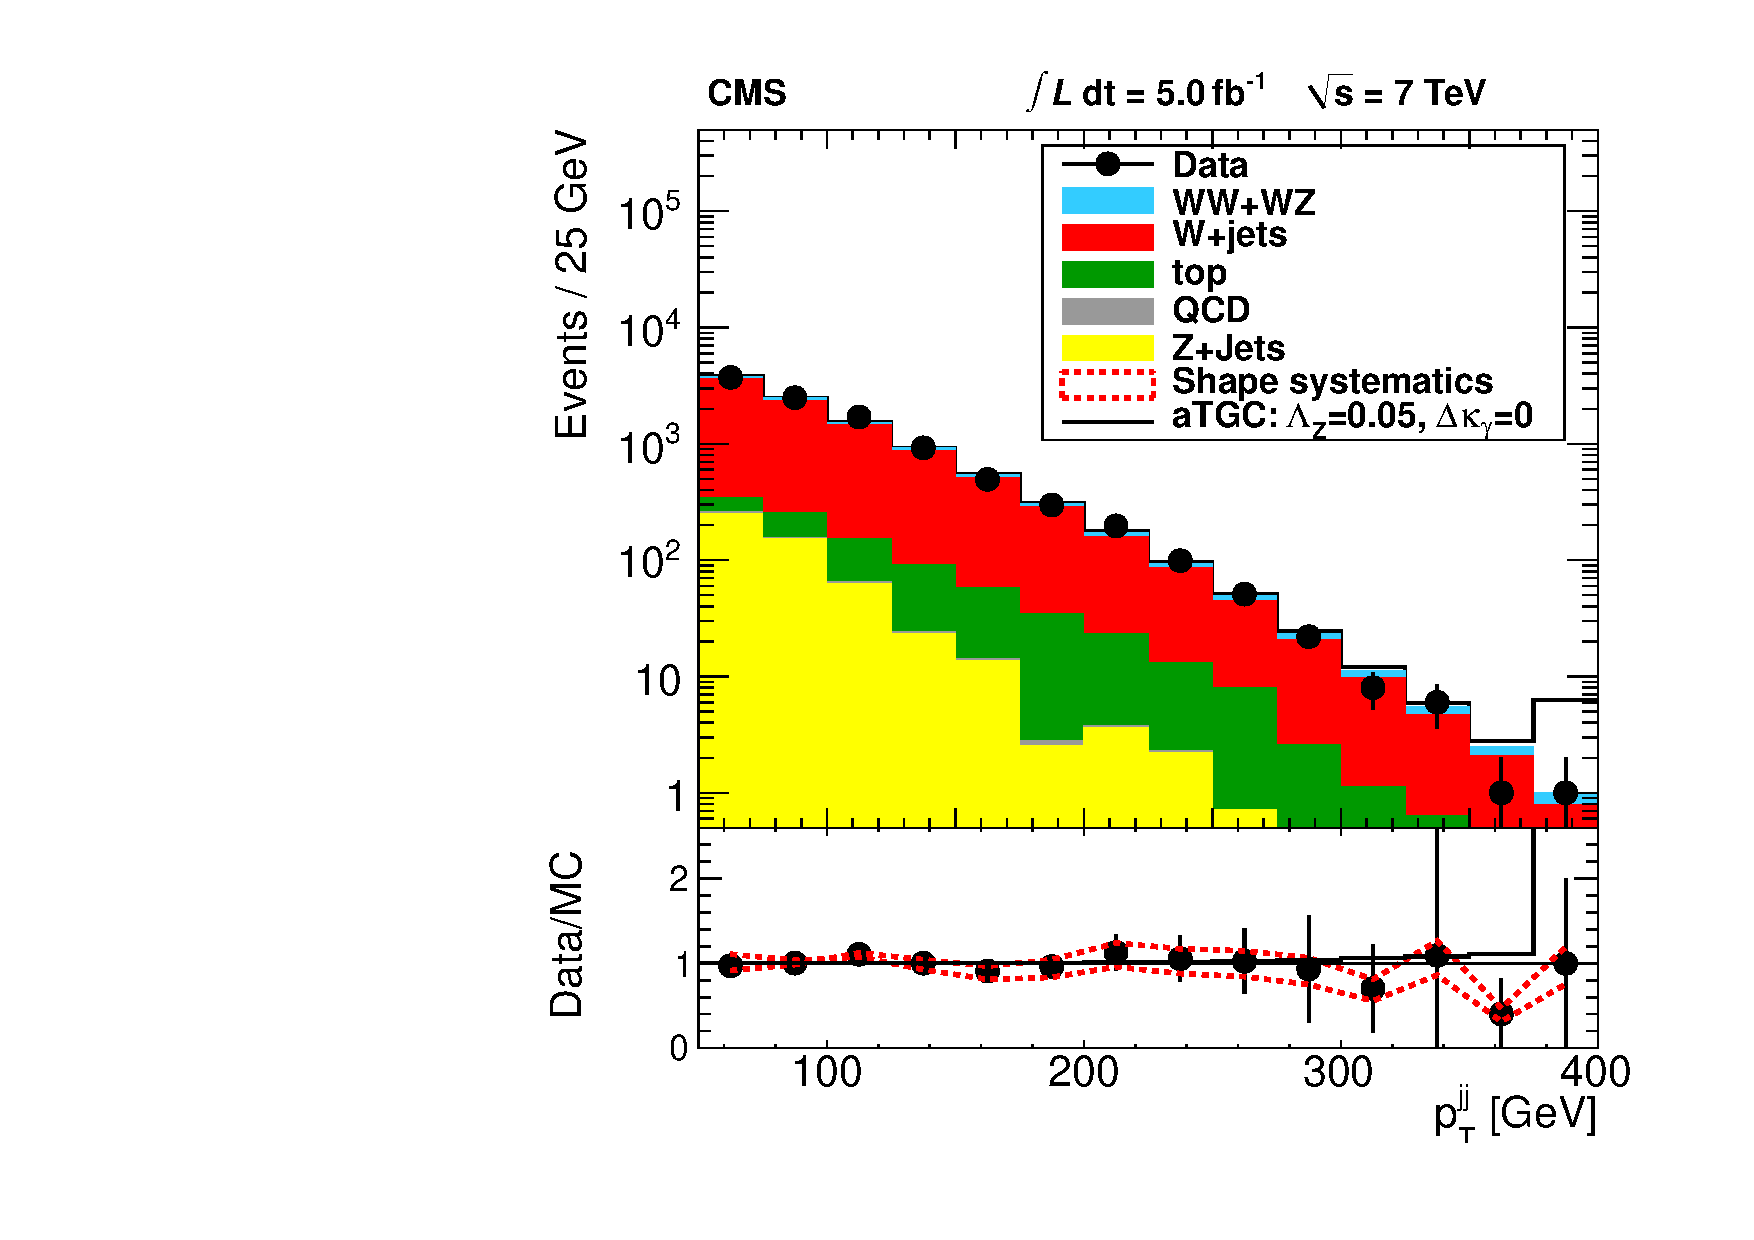
\includegraphics[width=0.4\textwidth]{figs/mu_noBtag_dijetPt.pdf}
    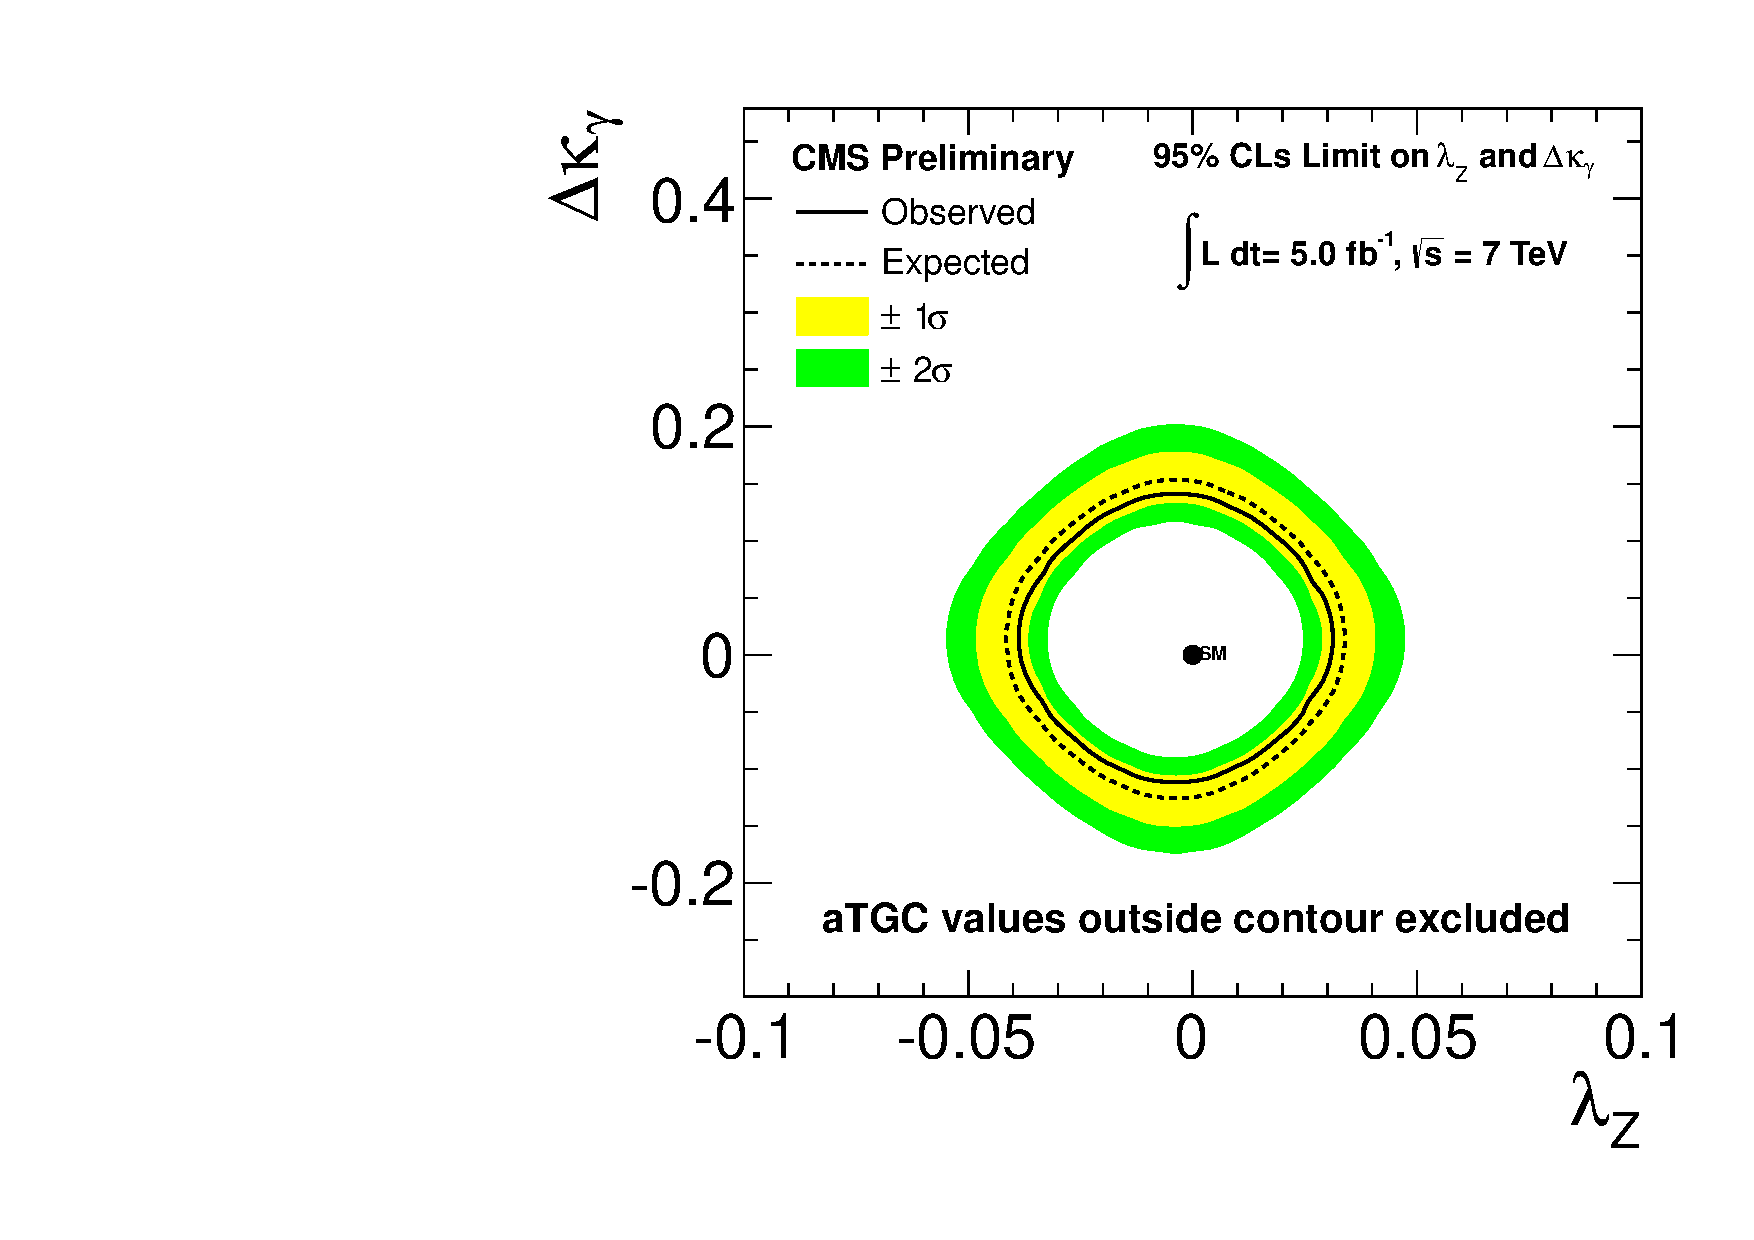
\includegraphics[width=0.4\textwidth]{figs/atgc_limits_withshape_contours.pdf}
    \caption{(a) Dijet $p_T$ distribution for muon no b-tag category  after requiring 
    $75~\GeVnn < \mjj < 95~\GeVnn$ (b)
 The observed and expected values of the upper limit for 
anomalous triple gauge couplings after combining results of all four event categories.
    }
    \label{fig:Fig2}}
\end{figure}
%%%%%%%%%%%%%%%%%%%%%%%%%%%%

% >> acknowledgements (for journal papers)
% Please include the latest version from https://twiki.cern.ch/twiki/bin/viewauth/CMS/Internal/PubAcknow.
%\section*{Acknowledgements}
% ack-text

%% **DO NOT REMOVE BIBLIOGRAPHY**
\bibliography{auto_generated}   % will be created by the tdr script.

%%% DO NOT ADD \end{document}!

